While scalability is the major benefit of local Lagrangian flow maps, this benefit comes with certain limitations as shown in our evaluation.
%
%First, as observed for the Jet data set, a vector field with very high velocity might be poorly reconstructed.
%
%In particular, we observe this for the Jet data set.
%
Lagrangian$_{Local}$ reconstruction accuracy can be adversely affected if the storage interval is too large or if too few samples are stored.
%
%This limits the potential amount of data reduction in comparison to Lagrangian$_{Dist}$.
%
%is effective for several practical configurations, the accuracy suffers when a large percentage of particles 
%is less accurate than Lagrangian$_{Dist}$ when the storage interval is large or the number of particles used to sample the domain is small, i.e., it limits the degree of data reduction.
%
%Prior works have demonstrated that Lagrangian$_{Dist}$ can provide high accuracy while using a small number of samples. 
%, i.e., providing a significant data reduction (for example, 1:64 data reduction factor corresponds to a $>$98\% compression of time-varying vector data).
%
%The Lagrangian$_{Local}$ strategy leverages this knowledge and discards particle trajectories in order to remain communication-free.
%
%However, this strategy is only effective as long as Lagrangian$_{Local}$ still stores a sufficient number of samples. 
%
While both Lagrangian$_{Dist}$ and Lagrangian$_{Local}$ show error (as shown in Figure~\ref{fig:strongscaling}), the error of Lagrangian$_{Local}$ increases faster when using a small number of samples or large storage intervals.
%

We briefly discuss two solutions to these challenges.
%
%The first potential solution is to detect high velocity regions, and adapt execution to adopt some local communication with spatially adjacent ranks.
The first potential solution is adapt execution to adopt some local communication with spatially adjacent ranks.
%
%Infrequent global communication would then also be required to exchange particles before storing to disk.
%Such a technique can be triggered if high velocity regions are detected.
%For example, the Los Alamos National Laboratory MPAS-O uses an integrated online Lagrangian analysis system that uses a combination of frequent local communication and infrequent global communication to perform particle exchange operations~\cite{VANSEBILLE201849}.
%
%However, we are unaware of technical details or a study of this system and expect its performance would be dependent on the specific application (underlying vector field), domain decomposition, rank placement, and synchronization.
%
The second solution is to stop discarding trajectories that hit the domain boundary, and instead utilize them for reconstruction. 
%
In this case, Lagrangian analysis could remain communication-free but would need enhancements not only for how to represent trajectories (termination location and time, number of points stored along pathline), but also would require a novel post hoc interpolation scheme.
%
\fix{For example, extensions of recent works on in situ sampling strategies~\cite{sane2019interpolation, rapp2019void} and post hoc reconstruction leveraging deep learning~\cite{jakob2020fluid} offer potential solutions.}
%
%In this case, Lagrangian analysis would remain communication-free but would need enhancements not only for how to represent trajectories that end abruptly (location, time, number of points along the curve, etc.) involves Lagrangian analysis remaining communication-free while adopting a more complex strategy for domain coverage with particle termination information (location, time) stored.
%
%A flow map with arbitrary termination times for particle trajectories, however, would require a novel post hoc interpolation scheme.
%

\fix{Another challenge for Lagrangian analysis is adaptively determining the appropriate storage interval. 
%
Determining the temporal sampling rate on a per particle basis could offer improved data reduction propositions and greater temporal resolution for reconstruction.
%
Further, motivated by our results and to limit uncertainty, we believe it would be worthwhile to investigate time-varying flow visualization techniques that utilize individual intervals of Lagrangian flow maps.
%
Lastly, our paper presented a study that considered the entire flow field without an analysis of specific features.
%
Research understanding the uncertainty introduced by various reduced representations~(Eulerian, Lagrangian, ZFP, etc.) when reconstructing specific features of interest would be valuable to the visualization community.
%
We believe these challenges should be pursued for future work. 
%
That said, we believe a number of use cases for Lagrangian analysis in practice today could benefit from flow maps extracted using a communication-free model.}
\begin{figure}[!t]
\centering
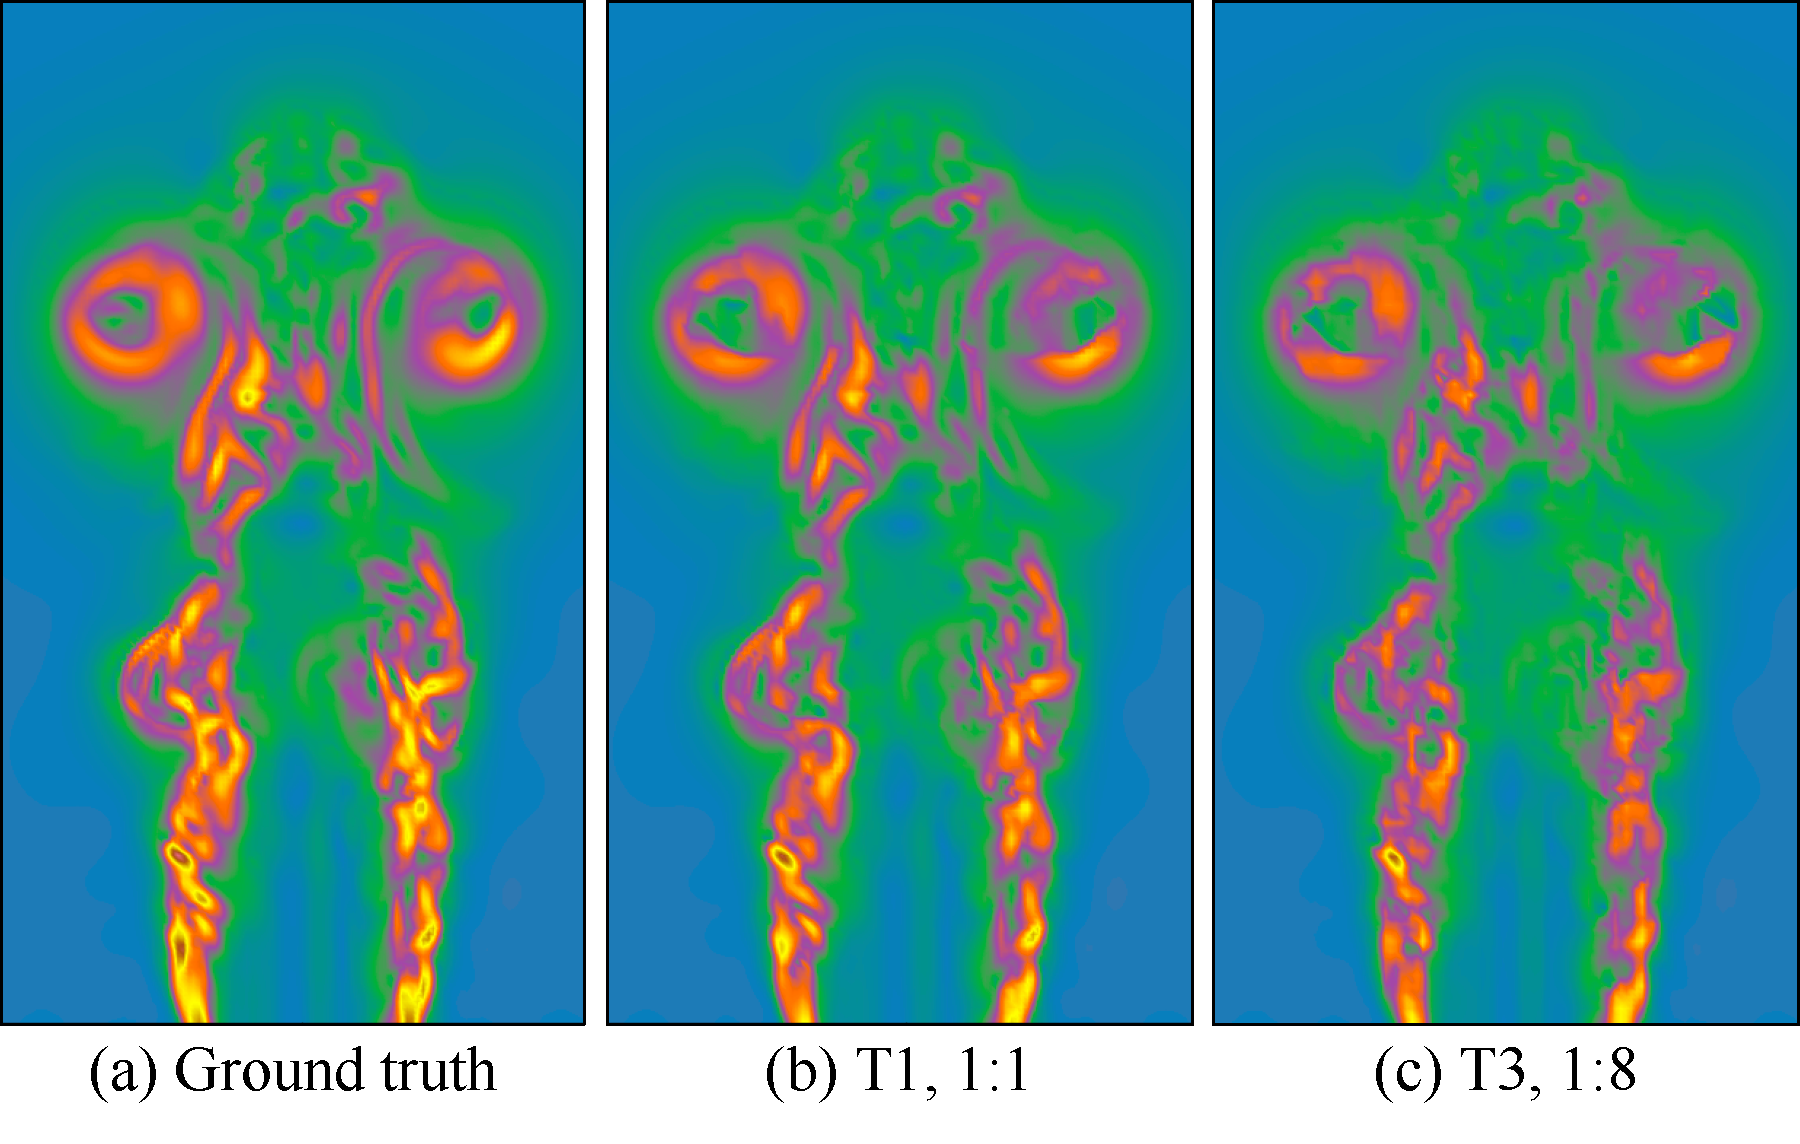
\includegraphics[width=\linewidth,keepaspectratio]{Images/jet_ftle_new.pdf}
\vspace{-5mm}
\caption{\fix{2D colormapped slices of the FTLE field computed over 5 cycles for the Jet data set. In both cases (b, c), flow maps over a single interval of Lagrangian$_{Local}$ are interpolated.}}
\vspace{-6mm}
\label{jet_ftle}
\end{figure}


